\section{eo\-Neg\-Exp\-Generator$<$ T $>$ Class Template Reference}
\label{classeo_neg_exp_generator}\index{eoNegExpGenerator@{eoNegExpGenerator}}
The class {\bf negexp\_\-generator}{\rm (p.\,\pageref{classnegexp__generator})} can be used in the STL generate function to easily generate negative exponential distributed floats and doubles.  


{\tt \#include $<$eo\-Rnd\-Generators.h$>$}

Inheritance diagram for eo\-Neg\-Exp\-Generator$<$ T $>$::\begin{figure}[H]
\begin{center}
\leavevmode
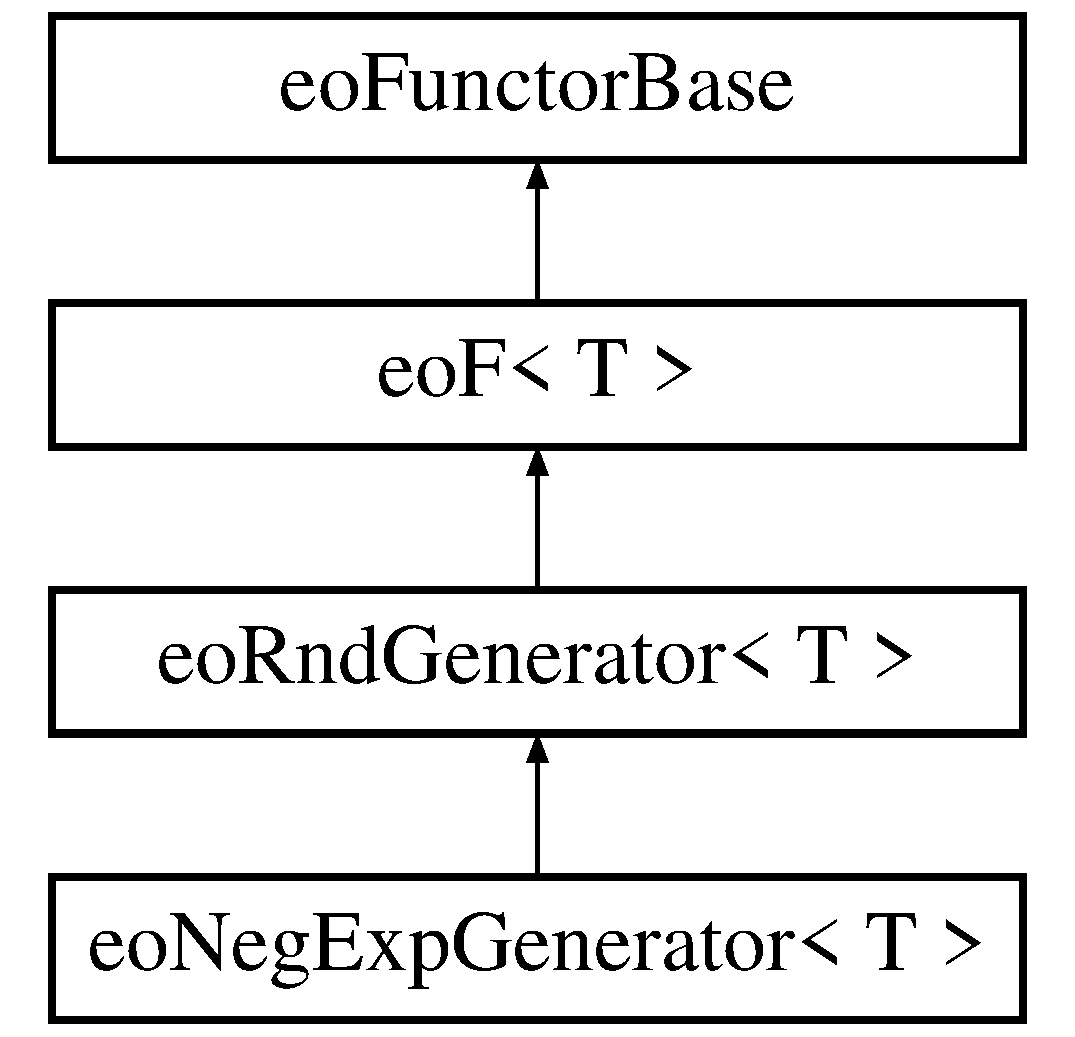
\includegraphics[height=4cm]{classeo_neg_exp_generator}
\end{center}
\end{figure}
\subsection*{Public Member Functions}
\begin{CompactItemize}
\item 
{\bf eo\-Neg\-Exp\-Generator} (T \_\-mean=1.0, {\bf eo\-Rng} \&\_\-rng=rng)\label{classeo_neg_exp_generator_a0}

\item 
T {\bf operator()} (void)\label{classeo_neg_exp_generator_a1}

\begin{CompactList}\small\item\em The pure virtual function that needs to be implemented by the subclass. \item\end{CompactList}\end{CompactItemize}
\subsection*{Private Attributes}
\begin{CompactItemize}
\item 
T {\bf mean}\label{classeo_neg_exp_generator_r0}

\item 
{\bf eo\-Rng} \& {\bf negexp}\label{classeo_neg_exp_generator_r1}

\end{CompactItemize}


\subsection{Detailed Description}
\subsubsection*{template$<$class T = double$>$ class eo\-Neg\-Exp\-Generator$<$ T $>$}

The class {\bf negexp\_\-generator}{\rm (p.\,\pageref{classnegexp__generator})} can be used in the STL generate function to easily generate negative exponential distributed floats and doubles. 

The user can supply a mean. 



Definition at line 137 of file eo\-Rnd\-Generators.h.

The documentation for this class was generated from the following file:\begin{CompactItemize}
\item 
eo\-Rnd\-Generators.h\end{CompactItemize}
